
\documentclass[a4paper,11pt]{article}
\usepackage[a4paper, margin=8em]{geometry}

% usa i pacchetti per la scrittura in italiano
\usepackage[french,italian]{babel}
\usepackage[T1]{fontenc}
\usepackage[utf8]{inputenc}
\frenchspacing 

% usa i pacchetti per la formattazione matematica
\usepackage{amsmath, amssymb, amsthm, amsfonts}

% usa altri pacchetti
\usepackage{gensymb}
\usepackage{hyperref}
\usepackage{standalone}

% imposta il titolo
\title{Appunti Elettronica Digitale}
\author{Luca Seggiani}
\date{2026}

% imposta lo stile
% usa helvetica
\usepackage[scaled]{helvet}
% usa palatino
\usepackage{palatino}
% usa un font monospazio guardabile
\usepackage{lmodern}

\renewcommand{\rmdefault}{ppl}
\renewcommand{\sfdefault}{phv}
\renewcommand{\ttdefault}{lmtt}

% disponi il titolo
\makeatletter
\renewcommand{\maketitle} {
	\begin{center} 
		\begin{minipage}[t]{.8\textwidth}
			\textsf{\huge\bfseries \@title} 
		\end{minipage}%
		\begin{minipage}[t]{.2\textwidth}
			\raggedleft \vspace{-1.65em}
			\textsf{\small \@author} \vfill
			\textsf{\small \@date}
		\end{minipage}
		\par
	\end{center}

	\thispagestyle{empty}
	\pagestyle{fancy}
}
\makeatother

% disponi teoremi
\usepackage{tcolorbox}
\newtcolorbox[auto counter, number within=section]{theorem}[2][]{%
	colback=blue!10, 
	colframe=blue!40!black, 
	sharp corners=northwest,
	fonttitle=\sffamily\bfseries, 
	title=~\thetcbcounter: #2, 
	#1
}

% disponi definizioni
\newtcolorbox[auto counter, number within=section]{definition}[2][]{%
	colback=red!10,
	colframe=red!40!black,
	sharp corners=northwest,
	fonttitle=\sffamily\bfseries,
	title=~\thetcbcounter: #2,
	#1
}

% U.D.M
\newcommand{\amp}{\ensuremath{\mathrm{A}}}
\newcommand{\volt}{\ensuremath{\mathrm{V}}}
\newcommand{\meter}{\ensuremath{\mathrm{m}}}
\newcommand{\second}{\ensuremath{\mathrm{s}}}
\newcommand{\farad}{\ensuremath{\mathrm{F}}}
\newcommand{\henry}{\ensuremath{\mathrm{H}}}
\newcommand{\siemens}{\ensuremath{\mathrm{S}}}

% circuiti
\usepackage{circuitikz}
\usetikzlibrary{babel}

% disegni
\usepackage{pgfplots}
\pgfplotsset{width=10cm,compat=1.9}

% disponi codice
\usepackage{listings}
\usepackage[table]{xcolor}

\definecolor{codegreen}{rgb}{0,0.6,0}
\definecolor{codegray}{rgb}{0.5,0.5,0.5}
\definecolor{codepurple}{rgb}{0.58,0,0.82}
\definecolor{backcolour}{rgb}{0.95,0.95,0.92}

\lstdefinestyle{codestyle}{
		backgroundcolor=\color{black!5}, 
		commentstyle=\color{codegreen},
		keywordstyle=\bfseries\color{magenta},
		numberstyle=\sffamily\tiny\color{black!60},
		stringstyle=\color{green!50!black},
		basicstyle=\ttfamily\footnotesize,
		breakatwhitespace=false,         
		breaklines=true,                 
		captionpos=b,                    
		keepspaces=true,                 
		numbers=left,                    
		numbersep=5pt,                  
		showspaces=false,                
		showstringspaces=false,
		showtabs=false,                  
		tabsize=2
}

\lstdefinestyle{shellstyle}{
		backgroundcolor=\color{black!5}, 
		basicstyle=\ttfamily\footnotesize\color{black}, 
		commentstyle=\color{black}, 
		keywordstyle=\color{black},
		numberstyle=\color{black!5},
		stringstyle=\color{black}, 
		showspaces=false,
		showstringspaces=false, 
		showtabs=false, 
		tabsize=2, 
		numbers=none, 
		breaklines=true
}

\lstdefinelanguage{javascript}{
	keywords={typeof, new, true, false, catch, function, return, null, catch, switch, var, if, in, while, do, else, case, break},
	keywordstyle=\color{blue}\bfseries,
	ndkeywords={class, export, boolean, throw, implements, import, this},
	ndkeywordstyle=\color{darkgray}\bfseries,
	identifierstyle=\color{black},
	sensitive=false,
	comment=[l]{//},
	morecomment=[s]{/*}{*/},
	commentstyle=\color{purple}\ttfamily,
	stringstyle=\color{red}\ttfamily,
	morestring=[b]',
	morestring=[b]"
}

% disponi sezioni
\usepackage{titlesec}

\titleformat{\section}
	{\sffamily\Large\bfseries} 
	{\thesection}{1em}{} 
\titleformat{\subsection}
	{\sffamily\large\bfseries}   
	{\thesubsection}{1em}{} 
\titleformat{\subsubsection}
	{\sffamily\normalsize\bfseries} 
	{\thesubsubsection}{1em}{}

% disponi alberi
\usepackage{forest}

\forestset{
	rectstyle/.style={
		for tree={rectangle,draw,font=\large\sffamily}
	},
	roundstyle/.style={
		for tree={circle,draw,font=\large}
	}
}

% disponi algoritmi
\usepackage{algorithm}
\usepackage{algorithmic}
\makeatletter
\renewcommand{\ALG@name}{Algoritmo}
\makeatother

% disponi numeri di pagina
\usepackage{fancyhdr}
\fancyhf{} 
\fancyfoot[L]{\sffamily{\thepage}}

\makeatletter
\fancyhead[L]{\raisebox{1ex}[0pt][0pt]{\sffamily{\@title \ \@date}}} 
\fancyhead[R]{\raisebox{1ex}[0pt][0pt]{\sffamily{\@author}}}
\makeatother

\begin{document}
% sezione (data)
\section{Lezione del 20-03-26}

% stili pagina
\thispagestyle{empty}
\pagestyle{fancy}

% testo
Veniamo a come regolare la tensione usando i diodi Zener.

\subsubsection{Lavorare in breakdown}
Poniamo il seguente circuito, formato du un diodo di zener sottoposto ad un certo voltaggio $V_2$ in polarizzazione inversa. Viene da sé che questo verrà messo a valle del circuito rettificatore filtrato RC che abbiamo visto alla fine della scorsa lezione.
\begin{center}
	\begin{tikzpicture}
		\draw (0,0) to [ battery2,  l=$V_2$] (0,3)
			to [ resistor, l=$R$] (3,3);
		\draw (3,0) to [ zD ] (3,3);
		\draw (3,0) -- (0,0);
		\node at(3,2.25) [anchor=west] {$K$};
		\node at(3,0.75) [anchor=west] {$A$};
	\end{tikzpicture}
\end{center}
In questo caso $V_2$ sarà una tensione con una componente DC, che vogliamo isolare dal resto del segnale (rumore, e nel contesto dei rettificatori di cui parlavamo alla scorsa lezione, \textit{ripple} voltage).

Prendiamo quindi la retta di carico (considerata per la prima volta in 6.1.3 nello studio del diodo), che sarà:
$$
I_D = -\frac{V_2 + V_D}{R}
$$
in quanto il diodo zener è in polarizzazione negativa rispetto a $V_2$. Abbiamo quindi una retta la cui intercetta alle ascisse è variata da $V_2$, mentre il coefficiente angolare è variato da $R$.
Su un grafico, essa appare come:
\begin{center}
	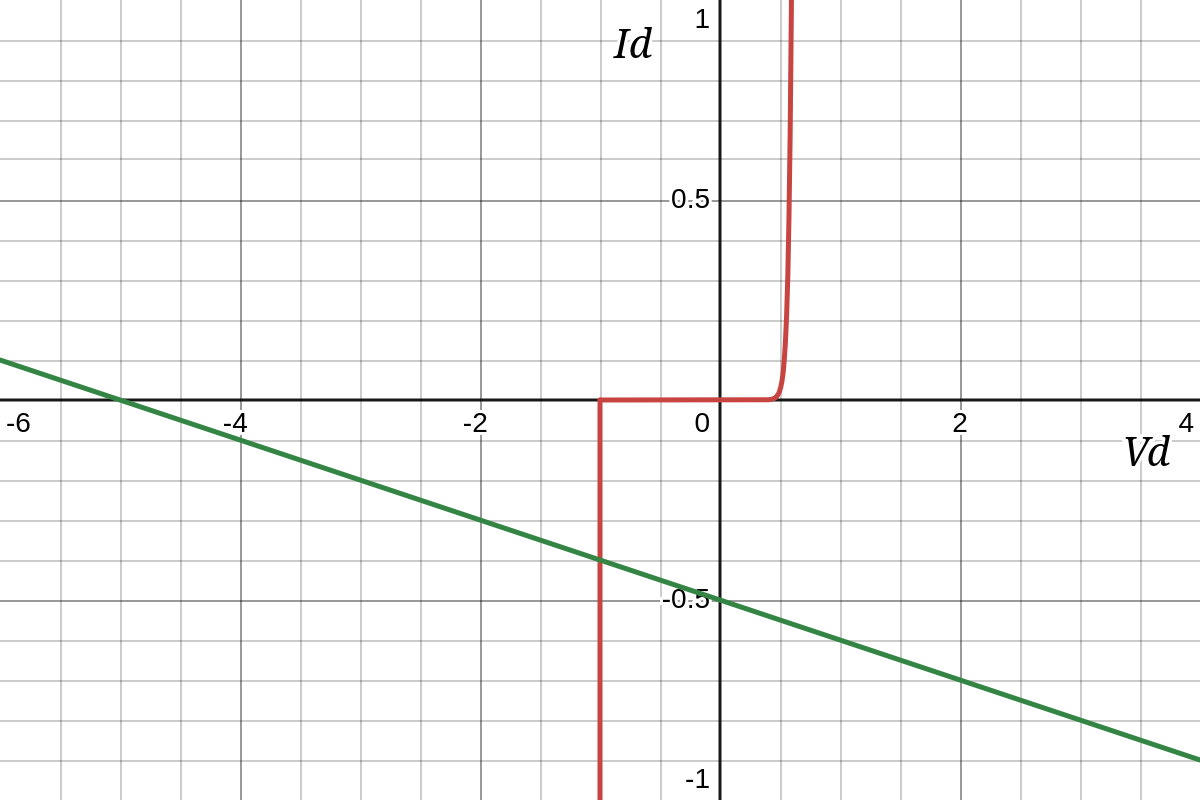
\includegraphics[scale=0.25]{../figures/zener_reg.png}
\end{center}
cioè per qualsiasi valore di $V_D$ negativa oltre la $V_Z$ di breakdown imposta sullo zener, questo esprimerà una corrente costante (pari a $V_Z$).

Per facilitare l'analisi, indichiamo $I_Z = -I_D$. Notiamo che, come sempre, vale:
$$
P_Z = V_Z I_Z
$$

Sarà quindi che la potenza dissipata sul diodo è il prodotto fra la corrente che ci passa e la tensione dissipata. Usando diodi zener, che lavorano in regioni dove la corrente può crescere anche molto, dobbiamo stare attenti a mantenere $P_Z$ entro le soglie di operatività dello zener. Altrimenti si avrebbero aumenti della temperatura, che da quanto discusso parlando delle giunzioni PN sappiamo ci porteranno a fallimento del diodo.

\subsubsection{Rettificatore con regolatore di tensione}
Possiamo quindi completare il design del nostro rettificatore introducendo il circuito di regolazione della tensione che abbiamo appena studiato. Questo porterò al seguente schema:
\begin{center}
\scalebox{0.8}{
\begin{circuitikz}
	\draw (-5, 2) -- (-2, 2);
	\draw (2, 2) -- (3, 2) -- (3, -2) -- (-5, -2);
	\draw (0, 0) -- (8, 0);
	\draw (0, 4) -- (5, 4);

	\draw (-2, 2) to[diode, l=$D_1$] (0, 4);
	\draw (0, 0) to[diode, l=$D_2$] (-2, 2);
	\draw (0, 0) to[diode, l_=$D_3$] (2, 2);
	\draw (2, 2) to[diode, l_=$D_4$] (0, 4);

	\draw (-5, 2) to[american voltage source, l=$V_s$] (-5, -2);
	\draw (5, 4) to[capacitor, l=$C$] (5, 0);
	\node[ground] at(5,0) {};
	\draw (5, 4) to[resistor, l=$R$] (8, 4);
	\draw (8,0) to[zD] (8, 4);
	\draw (8,4) -- (11, 4) to[resistor, l=$R_L$] (11, 0) -- (8, 0);
	\draw (11, 4) -- (12, 4);
	
	\node[anchor=west] at(12,4) {$V_u$};

	\node[anchor=north] at(4,4) {$+$};
	\node at(4,2) {$V_2$};
	\node[anchor=south] at(4,0) {$-$};
\end{circuitikz}
}
\end{center}

Lo scopo del componente che abbiamo aggiunto, cioè la coppia $R$ (che si va a differenziare dalla $R_L$ di carico) e diodo di zener, è quello di regolare la tensione $V_2$ (quella in uscita dal ponte di Graetz filtrato RC, cioè la tensione sulla capacità C).

Per studiare tale circuito facciamo l'ipotesi che lo zener lavori in breakdown, cioè:
$$
I_Z > 0 \implies V_u = V_Z
$$
e quindi la tensione in uscita dal circuito $V_u$ è pari alla tensione di breakdown $V_Z$ del diodo.

\par\smallskip

\noindent
\textbf{\textsf{Verifica}}

\noindent
Questo si verifica calcolando la corrente sullo zener, in modo da verificare che questo si trovi in regime di breakdown (corrente negativa):
$$
I_R = \frac{V_2 - V_Z}{R}, \quad I_L = \frac{V_Z}{R_L} \implies I_Z = I_R - I_L = \frac{V_2 - V_Z}{R} - \frac{V_Z}{R_L} > 0
$$
dove $I_R$ è la corrente sulla resistenza $R$ diretta verso destra , $I_L$ è la corrente sulla resistenza di carico $R_L$ diretta verso il basso. Da quanto detto prima rispetto allo zener, $I_Z = I_R - I_L$ è un'affermazione della prima legge di Kirchoff.

Abbiamo quindi imposto la $I_Z > 0$, che era la nostra ipotesi di funzionamento del diodo in regime di breakdown. Nel caso in cui la disequazione non sia soddisfatta, significherà che non siamo riusciti a portare lo zener nel regime di breakdown, e quindi la tensione $V_u$ che misuriamo è nulla.

\par\smallskip

\noindent
\textbf{\textsf{Scelta della resistenza}}

\noindent
Interroghiamoci su come si andrà a scegliere la $R$ nel circuito di regolazione a diodo di zener. Questa resistenza è proprio quella che sta a limitare la $P_Z = V_Z I_Z$ dello scorso paragrafo, e quindi la corrente che scorre sul diodo. Vogliamo mantenere questa limitata in modo che il diodo operi nei suoi regimi validi.

Abbiamo che la tensione a valle del ponte di Graetz filtrato RC è soggetta a ripple, per cui possiamo dire:
$$
V_{2,\mathrm{min}} \leq V_2 \leq V_{2,\mathrm{max}}
$$

Nel caso peggiore, il carico non richiede corrente, per cui $R_L \rightarrow +\infty$, o anzi la sostituiamo direttamente con un aperto. In tal caso tutta la corrente si trova sul zener:
$$
I_{Z,\mathrm{max}} = \frac{V_{2,\mathrm{max}} - V_Z}{R} 
$$

Dal datasheet dello zener avremo una certa potenza $P_{Z,\mathrm{max}}$, che è la \textit{massima} tollerabile dal diodo. Imporremo quindi che tale potenza non venga superata:
$$
V_Z I_{Z,\mathrm{max}} < P_{Z,\mathrm{max}} \implies R^* > \frac{(V_{2,\mathrm{max}} - V_Z) V_Z}{P_{Z,\mathrm{max}}} 
$$
cioè $R^*$ sarà la resistenza \textit{minima} che potremmo mettere nel circuito regolatore in modo da evitare che questo bruci. 

Al carico $R_L$, invece, quando questo richiede corrente, avremo al limite $I_Z = 0$, per cui potremo offrire almeno la corrente $I_L$:
$$
I_{L,\mathrm{max}} = \frac{V_{2,\mathrm{min}} - V_Z}{R}
$$

\subsection{Modello del diodo ai piccoli segnali}
Finora abbiamo trattato il diodo ai grandi segnali, cioe per cadute di tensione $\Delta V >> V_\gamma \approx 0.7 \, \mathrm{V}$ o comunque confrontabili. Vediamo invece come trattare il diodo per i piccoli segnali, cioè quelli $\Delta V << V_\gamma$.

In tal caso riprenderemo la legge di Shockley, vista in 6.1, e quindi l'andamento esponenziale dela corrente sul diodo:
$$
I_D = I_S \left( e^{\frac{V_D}{\eta V_T}} - 1\right)
$$
dove $I_S$ era la corrente di saturazione, $\eta$ il fattore di idealità e $V_T$ la tensione termica.
Per un piccolo segnale è inutile prendere l'intero esponenziale, e si può invece prendere un punto centrale $Q$ e linearizzare la risposta attorno ad esso.

\begin{center}
	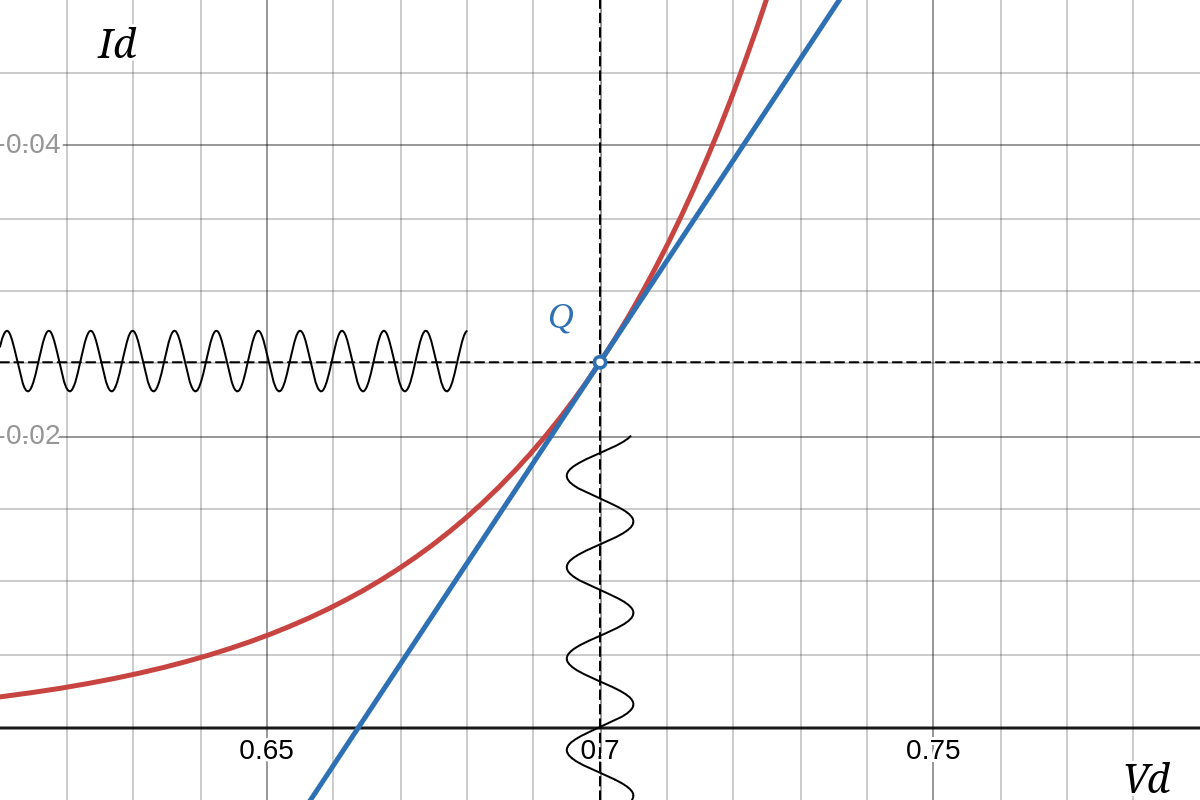
\includegraphics[scale=0.25]{../figures/linearized_diode.png}
\end{center}

Più nel dettaglio, se le variazioni del segnale ($v_d(t)$) sono sufficientemente piccole rispetto alla tensione termica ($V_T$), la curva esponenziale del diodo può essere approssimata con un segmento rettilineo (la tangente nel punto $Q$, dove $Q$ sta per \textit{Quiescenza}).
In questo modo potremo dire che esiste una legge del tipo:
$$
\begin{cases}
V_D(t) = V_{DQ} + v_d(t) \\
I_D(t) = I_{DQ} + i_d(t)
\end{cases}
$$
per tensione e corrente sul diodo in relazione a $Q$.

Questo ci dà due vantaggi:
\begin{enumerate}
	\item \textbf{Semplificazione} del circuito: anziché risolvere equazioni trascendentali, cioè la funzione esponenziale, trattiamo il diodo come una semplice resistenza $r_d$, con:
$$
i_d = g_d v_d, \quad v_d = r_d i_d \quad \text{con} \quad r_d = \frac{1}{g_d}
$$
dove la $g_d$ (la \textit{conduttività} dell'approssimazione a resistenza) non è altro che la pendenza della retta linearizzante;
\item Inoltre, sfruttare un modello linearizzato ci permette di applicare il principio di \textbf{sovrapposizione} degli effetti. In altre parole, in un circuito linearizzato, possiamo separare nettamente l’analisi in continua (che fissa il punto $Q$ di quiescenza) dall’analisi in alternata (che elabora il segnale).
\end{enumerate}

\par\smallskip

\noindent
\textbf{\textsf{Linearizzazione su $\mathbf{Q}$}}

\noindent
Vediamo quindi a come ricavare i valori linearizzati, cioè ricaviamoci espressioni esplicite per $V_{DQ}$, $I_{DQ}$ e la conduttanza $g_d$ ($r_d$ è facilmente ricavabile da $\frac{1}{g_d}$).

Per fare ciò prendiamo lo sviluppo di Taylor attorno a $Q$ dell'equazione di Shockley, che chiamiamo $S(V_D)$:
$$
I_D(t) = S(V_D(t)) = S(Q + v_d(t)) = S(Q) + \frac{\partial}{\partial V_D} S(Q) v_d(t) + \frac{1}{2} \frac{\partial^2}{\partial V_D^2} S(Q) v_d^2(t) + ...
$$
e tronchiamo al termine lineare, cioè:
$$
\approx S(Q + v_d(t)) = S(Q) + \frac{\partial}{\partial V_D} S(Q) v_d(t)
= I_{DQ} + g_d v_d(t) = I_{DQ} + i_d(t)
$$
Abbiamo quindi la forma linearizzata di $I_D(t)$, dove notiamo:
$$
I_{DQ} = S(Q), \quad i_d(t) = g_d v_d(t)
$$
Allo stesso modo, per come abbiamo scelto $Q$, potremo dire che semplicemente:
$$
V_{DQ} = Q, \quad v_d(t) = r_d i_d(t)
$$
In genere vale poi:
$$
g_d = \frac{\partial}{\partial V_D} S(Q), \quad r_d = \frac{1}{g_d} = \left( \frac{\partial}{\partial V_D} S(Q) \right)^{-1}
$$
chiamate rispettivamente \textit{conduttanza differenziale} e \textit{resistenza differenziale}.

\newpage

Questa selezione di variabili ci assicura che:
\begin{enumerate}
	\item Prendiamo il comportamento su $Q \rightarrow S(Q)$, cioè $V_{DQ} \rightarrow I_{DQ}$, e lo fissiamo come contributo costante;
	\item Troviamo espressioni dei piccoli segnali $v_d(t)$ e $i_d(t)$ che permettono di trattare il diodo come un resistore a conduttanza $g_d$;
	\item Sommare il contributo DC $I_{DQ}$ al piccolo segnale $i_d(t)$ dà un espressione valida per la corrente sul diodo $I_D(t)$, e allo stesso modo $V_{DQ}$ più il piccolo segnale $v_d(t)$ dà un espressione valida per la tensione sul diodo $V_D(t)$. Queste espressioni valide sono poi le stesse di prima:
$$
\begin{cases}
I_D(t) = I_{DQ} + i_d(t) \\
V_D(t) = V_{DQ} + v_d(t)
\end{cases}
$$
e siamo felici.
\end{enumerate}

\par\smallskip

\noindent
\textbf{\textsf{Collegamento alla legge di Shockley}}

\noindent
Smettiamo quindi di parlare della $S(V_D)$, e riprendiamo l'espressione propria della legge di Shockley:
$$
I_D = I_S \left( e^{\frac{V_D}{\eta V_T}} - 1\right)
$$

Ciò che vogliamo fare è trovare espressioni per $I_{DQ}$, $V_{DQ}$ e $g_d$ (come prima, $r_d$ è diretta da $g_d$) che derivino dai parametri della legge di Shockley (cioè la corrente di saturazione $I_S$, il fattore di idealità $\eta$, e la tensione termica $V_T$).

\begin{itemize}
	\item $V_{DQ}$ è banale in quanto è semplicemente la tensione di linearizzazione $Q$ (dovremmo ormai aver capito che $Q$ è una tensione e $V_{DQ} = Q$);
	\item $I_{DQ}$ si ricava abbastanza facilmente dalla legge di Shockley stessa, per cui:
$$
I_{DQ} = I_S \left( e^{\frac{Q}{\eta V_T}} - 1\right)
$$
	\item
Infine, $g_d$ era stata espressa come:
$$
g_d = \frac{\partial}{\partial V_D} S(Q) = \frac{\partial}{\partial V_D} I_S \left( e^{\frac{Q}{\eta V_T}} - 1\right)
$$
con $S$ la legge di Shockley. Dobbiamo quindi calcolare questa derivata:
$$
\frac{\partial}{\partial V_D} I_S \left( e^{\frac{V_D}{\eta V_T}} - 1\right) = 
\frac{I_S}{\eta V_T} e^{\frac{V_D}{\eta V_T}}
$$
per cui sostituendo $Q$ e ricordando $Q = V_{DQ}$ si ha:
$$
g_d = \frac{\partial}{\partial V_D} S(Q)=
\frac{I_S}{\eta V_T} e^{\frac{V_{DQ}}{\eta V_T}} = \frac{I_S \left( e^{\frac{V_D}{\eta V_T}} - 1 \right) + I_S }{\eta V_T} 
$$
$$
= \frac{I_{DQ} + I_S }{\eta V_T} \approx \frac{I_{DQ}}{\eta V_T}, \quad I_{DQ} >> I_S
$$
Quest'ultima espressione richiede alcune spiegazioni. Innanzitutto, il passaggio dove espandiamo la forma della derivata prima è matematicamente valido ($I_S$ si annulla con il $-1$). La semplificazione che facciamo in seguito, invece, vale quando $I_{DQ} >> I_S$, e ricordando che il termine a sinistra della somma è $I_{DQ}$ stesso.

Abbiamo quindi un espressione per $g_d$ in funzione del punto di linearizzazione. L'espressione di $r_d$ è immediata:
$$
g_d = \frac{I_{DQ}}{\eta V_T}, \quad r_d = \frac{\eta V_T}{I_{DQ}}
$$

\par\smallskip

\noindent
\textbf{\textsf{Verifica della validità}}

\noindent
Abbiamo trascurato i termini superiori nello sviluppo della serie di Taylor per poter linearizzare attorno a $Q$. Interroghiamoci iguardo alla validità di questa approssimazione. 
Di base, questa sarà valida se potremo dire:
$$
\left| \frac{\partial}{\partial V_D} S(Q) v_d(t) \right| >>
\left| \frac{1}{2} \frac{\partial^2}{\partial V_D^2} S(Q) v_d^2(t) \right|
$$
cioè il termine di primo grado è di molto maggiore rispetto al termine di secondo grado. Riportandoci al dominio delle derivate vere e proprie della legge di Shockley (non riportiamo il calcolo della derivata seconda in quanto tedioso):
$$
\frac{I_{DQ} + I_S}{\eta V_T} >> \frac{I_{DQ} + I_S}{2(\eta V_T)^2} \cdot |v_d(t)| \implies |v_d(t)| << 2 \eta V_T
$$

Abbiamo quindi ricavato una condizione perché la nostra approssimazione sia valida. A temperatura ambiente ($27^\circ \mathrm{C}$) si ha che:
$$
|v_d(t)| << 57.2 \,\mathrm{mV}
$$
cioè per segnali con ampiezze di pochi milli-volt la nostra approssimazione (linearizzazione) è valida.

\end{itemize}

\end{document}
